\documentclass[12pt,a4paper]{article}
\usepackage[utf8]{inputenc}
\usepackage[T1]{fontenc}
\usepackage[english]{babel}
\usepackage[left=2cm,right=2cm,top=2cm,bottom=2cm]{geometry}
\usepackage{lmodern}
\usepackage{amsmath}
\usepackage{amssymb}
\usepackage{physics}
\usepackage{booktabs}
\usepackage{tcolorbox}
\usepackage{siunitx}
\usepackage[table,xcdraw]{xcolor}
\usepackage{hyperref}
\usepackage{array}
\usepackage{textgreek}
\usepackage{fancyhdr}
\usepackage{enumitem}
\usepackage{graphicx}
\usepackage{float}
\usepackage{tikz}
\usepackage{braket}

% Color definitions
\definecolor{t0blue}{RGB}{0,102,204}
\definecolor{t0green}{RGB}{0,153,76}
\definecolor{t0red}{RGB}{204,0,51}
\definecolor{t0yellow}{RGB}{255,204,0}
\definecolor{t0purple}{RGB}{102,0,204}

% Header and Footer
\pagestyle{fancy}
\fancyhf{}
\fancyhead[L]{\color{t0blue}\textsc{T0 Theory: Resolution of Instantaneity}}
\fancyhead[R]{\color{t0blue}\textsc{Johann Pascher}}
\fancyfoot[C]{\thepage}
\renewcommand{\headrulewidth}{0.4pt}
\renewcommand{\footrulewidth}{0.4pt}

% Custom commands
\newcommand{\xipar}{\ensuremath{\xi}}
\newcommand{\Tfield}{\mathcal{T}}
\newcommand{\lP}{\ell_{\text{P}}}
\newcommand{\mP}{m_{\text{P}}}
\newcommand{\EP}{E_{\text{P}}}
\newcommand{\tP}{t_{\text{P}}}

% Hyperref settings
\hypersetup{
	colorlinks=true,
	linkcolor=t0blue,
	citecolor=t0blue,
	urlcolor=t0blue,
	pdftitle={T0 Theory: Resolution of Apparent Instantaneity},
	pdfauthor={Johann Pascher},
	pdfsubject={Theoretical Physics, T0 Theory, Quantum Mechanics},
	pdfkeywords={T0 Model, Instantaneity, Quantum Entanglement, Field Theory}
}

\title{{\Huge \color{t0blue}T0 Formalism}\\
	{\LARGE Complete Resolution of Apparent Instantaneity}\\
	\vspace{1cm}
	{\Large A Field-Theoretic Analysis of Causality in Quantum Mechanics}}
\author{{\Large Johann Pascher}\\
	Department of Communication Technology\\
	HTL Leonding, Austria\\
	\texttt{johann.pascher@gmail.com}}
\date{\today}

\begin{document}
	
	\maketitle
	\thispagestyle{empty}
	
	\begin{abstract}
		This work demonstrates that the apparent instantaneity in the T0 formalism arises from the notation of the local constraint condition $T \cdot E = 1$. Through analysis of the underlying field equations and hierarchical time scales, it is shown that T0 theory provides a completely causal description of quantum phenomena that is fully compatible with special relativity. All parameters of the theory follow from purely geometric principles. The work extends the analysis to the complete duality between time, mass, energy, and length, and critically discusses the limits of interpretation in extreme situations.
	\end{abstract}
	
	\newpage
	\hypersetup{linkcolor=blue}
	\tableofcontents
	\newpage
	
	\section{Introduction: The Instantaneity Problem}
	
	Since the groundbreaking work of Einstein, Podolsky, and Rosen in the 1930s, physics has struggled with a fundamental paradox: quantum mechanics appears to require instantaneous correlations between arbitrarily distant particles, which Einstein called ``spooky action at a distance.'' This apparent instantaneity manifests in various phenomena—from wave function collapse through Bell inequality violations to quantum entanglement.
	
	The T0 formalism offers an alternative resolution to this paradox. The core idea is that the fundamental relationship between time and energy, expressed by the equation $T \cdot E = 1$, is often misunderstood. What appears at first glance to be an instantaneous coupling proves upon closer examination to be a local constraint condition that implies no action at a distance.
	
	To understand this, we must distinguish between two fundamentally different types of physical relationships: local constraint conditions that apply at the same spatial point, and field equations that describe the propagation of disturbances through space. This distinction is the key to resolving the instantaneity paradox.
	
	\section{Apparent Instantaneity in the T0 Formalism}
	
	The T0 equations appear to imply instantaneity at first glance, but this is refuted through detailed analysis of the field equations. The fundamental challenge is understanding how a theory based on the strict relationship $T \cdot E = 1$ can nonetheless respect causality. This apparent paradox has its roots in a misunderstanding about the nature of mathematical constraint conditions in physics.
	
	\subsection{The Apparent Problem}
	
	The fundamental equations of the T0 formalism are:
	\begin{align}
		T(\mathbf{x},t) \cdot E(\mathbf{x},t) &= 1 \label{eq:TE_constraint} \\
		T &= \frac{1}{m} \quad \text{where } \omega = \frac{mc^2}{\hbar}, \text{ so } T = \frac{\hbar}{E} \label{eq:T_definition} \\
		E &= mc^2 \label{eq:E_definition}
	\end{align}
	
	These equations suggest that a change in $E$ requires an immediate adjustment of $T$. If we double the energy at a point, for example, the time field seems to have to halve instantaneously. This interpretation would indeed mean a violation of relativistic causality and stands in apparent contradiction to the fundamental principles of modern physics.
	
	The confusion arises from the fact that these equations are often interpreted as dynamic relationships—as if a change in one quantity causes an instantaneous reaction in the other. This interpretation is fundamentally wrong and leads to the apparent paradoxes of quantum mechanics.
	
	\subsection{The Resolution: Field Equations Have Dynamics}
	
	The resolution of this paradox lies in recognizing that the T0 equations contain two different types of relationships: local constraint conditions and dynamic field equations. This distinction is fundamental to understanding why no real instantaneity occurs.
	
	\textbf{1. The complete field equation:}
	\begin{equation}
		\nabla^2 m = 4\pi G \rho(\mathbf{x},t) \cdot m \label{eq:field_equation}
	\end{equation}
	where $\rho(\mathbf{x},t)$ is the mass density. This equation is \emph{not} instantaneous but rather a wave equation with finite propagation speed $v \leq c$.
	
	This field equation describes how disturbances in the mass field (and thus in the time field via $T = 1/m$) propagate through space. Crucially, this propagation occurs at finite speed, limited by the speed of light. The equation is second-order in spatial derivatives, which is characteristic of wave propagation. No information, no energy, and no effect can propagate faster than the speed of light.
	
	\textbf{2. The modified Schrödinger equation:}
	\begin{equation}
		i \cdot T(\mathbf{x},t) \frac{\partial \psi}{\partial t} = H_0 \psi + V_{T0} \psi \label{eq:schroedinger}
	\end{equation}
	where $H_0 = -\frac{\hbar^2}{2m}\nabla^2$ is the free Hamiltonian and $V_{T0} = \hbar^2 \delta E(\mathbf{x},t)$ is the T0-specific potential.
	
	This modified Schrödinger equation explicitly shows the temporal evolution of the wave function under the influence of the time field. The presence of the time derivative $\partial/\partial t$ makes clear that this is a causal evolution, not an instantaneous adjustment. The wave function evolves continuously in time according to local field conditions.
	
	\section{The Critical Insight: Local vs. Global Relations}
	
	The key to understanding lies in distinguishing between local and global physical relationships. This distinction is ubiquitous in physics but often not emphasized explicitly enough. The confusion between these two types of relationships is the source of many conceptual problems in quantum mechanics.
	
	\subsection{Visualization of Local vs. Global Relations}
	
	\begin{center}
		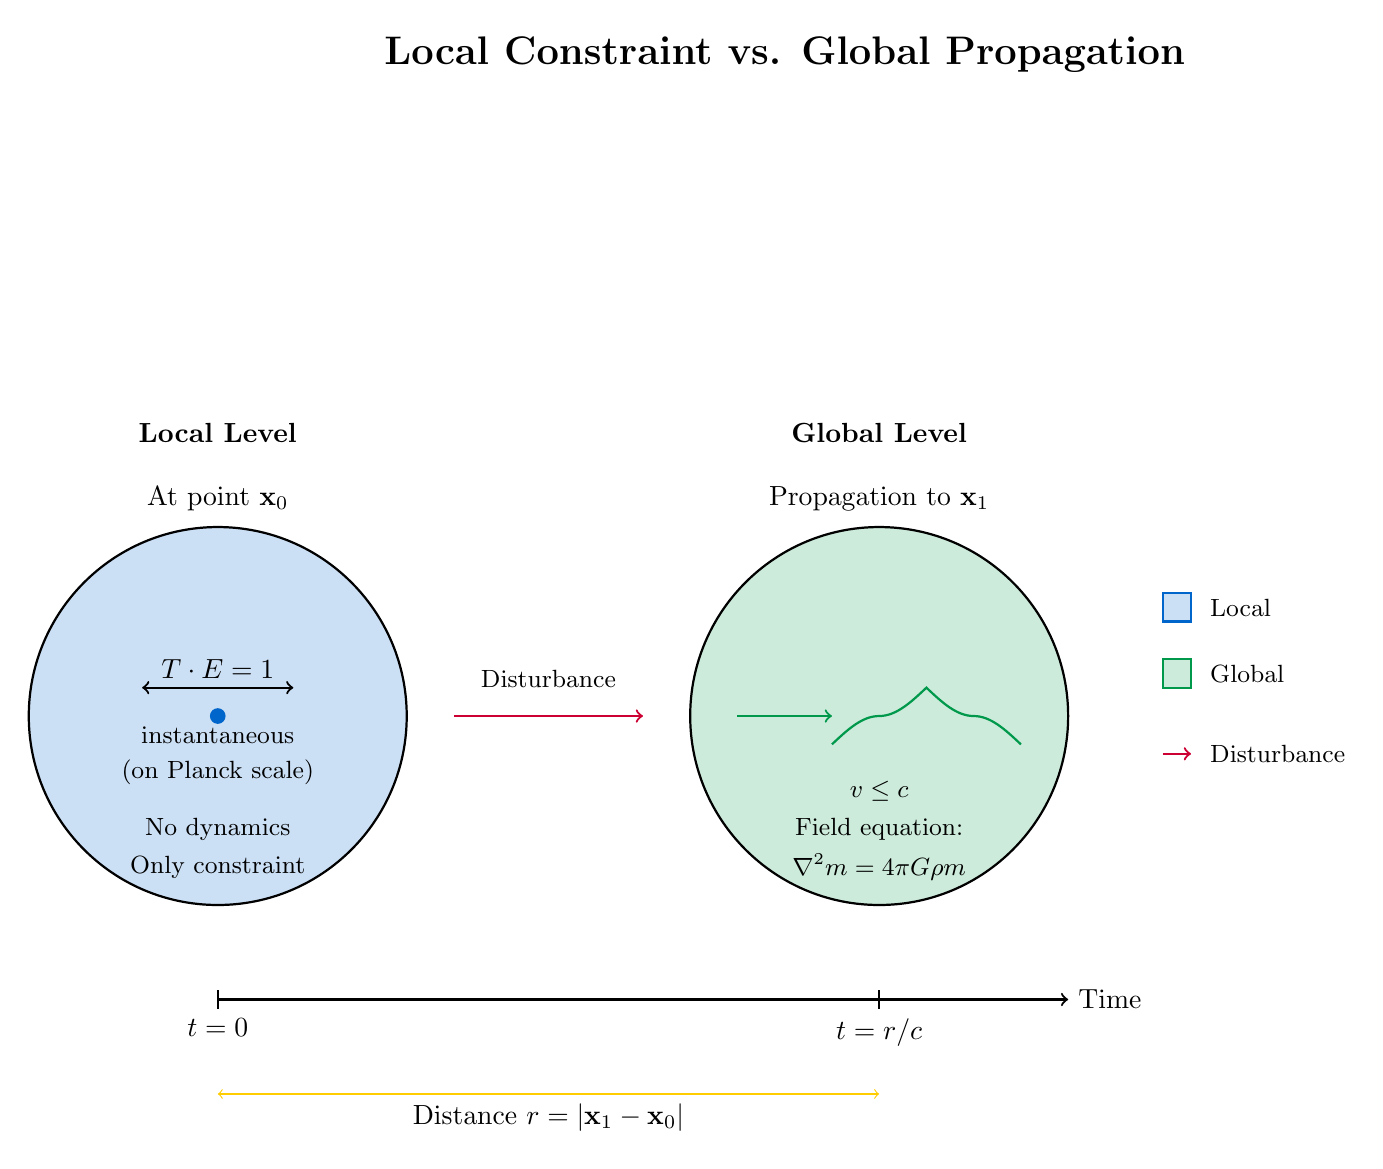
\begin{tikzpicture}[scale=1.2]
			% Title
			\node at (6, 7) {\Large \textbf{Local Constraint vs. Global Propagation}};
			
			% Local constraint (left)
			\draw[thick, fill=t0blue!20] (0,0) circle (2);
			\node at (0, 3) {\textbf{Local Level}};
			\node at (0, 2.3) {At point $\mathbf{x}_0$};
			\draw[thick, <->] (-0.8, 0.3) -- (0.8, 0.3);
			\node at (0, 0.5) {$T \cdot E = 1$};
			\node at (0, -0.2) {\small instantaneous};
			\node at (0, -0.6) {\small (on Planck scale)};
			\draw[thick, t0blue] (0,0) node[circle, fill, inner sep=2pt]{};
			\node at (0, -1.2) {\small No dynamics};
			\node at (0, -1.6) {\small Only constraint};
			
			% Arrow to the right
			\draw[thick, ->, t0red] (2.5, 0) -- (4.5, 0);
			\node[above] at (3.5, 0.2) {\small Disturbance};
			
			% Global propagation (right)
			\draw[thick, fill=t0green!20] (7,0) circle (2);
			\node at (7, 3) {\textbf{Global Level}};
			\node at (7, 2.3) {Propagation to $\mathbf{x}_1$};
			% Wave propagation
			\draw[thick, t0green, ->] (5.5, 0) -- (6.5, 0);
			\draw[thick, t0green] (6.5, -0.3) sin (7, 0) cos (7.5, 0.3) sin (8, 0) cos (8.5, -0.3);
			\node at (7, -0.8) {\small $v \leq c$};
			\node at (7, -1.2) {\small Field equation:};
			\node at (7, -1.6) {\small $\nabla^2 m = 4\pi G \rho m$};
			
			% Time axis below
			\draw[thick, ->] (0, -3) -- (9, -3) node[right] {Time};
			\draw[thick] (0, -3.1) -- (0, -2.9);
			\node[below] at (0, -3.1) {$t = 0$};
			\draw[thick] (7, -3.1) -- (7, -2.9);
			\node[below] at (7, -3.1) {$t = r/c$};
			
			% Distance
			\draw[<->, t0yellow] (0, -4) -- (7, -4);
			\node[below] at (3.5, -4) {Distance $r = |\mathbf{x}_1 - \mathbf{x}_0|$};
			
			% Legend
			\draw[thick, t0blue, fill=t0blue!20] (10, 1) rectangle (10.3, 1.3);
			\node[right] at (10.4, 1.15) {\small Local};
			\draw[thick, t0green, fill=t0green!20] (10, 0.3) rectangle (10.3, 0.6);
			\node[right] at (10.4, 0.45) {\small Global};
			\draw[thick, t0red, ->] (10, -0.4) -- (10.3, -0.4);
			\node[right] at (10.4, -0.4) {\small Disturbance};
		\end{tikzpicture}
	\end{center}
	
	This diagram illustrates the fundamental difference between local and global processes. On the left, we see the local constraint condition $T \cdot E = 1$, which holds instantaneously (on the Planck time scale) at the same spatial point. On the right, we see the global propagation of a disturbance, which occurs at finite speed $v \leq c$ and requires time $t = r/c$ to bridge the distance $r$.
	
	\subsection{Local Constraint Condition}
	
	\begin{equation}
		T(\mathbf{x},t) \cdot E(\mathbf{x},t) = 1 \quad \text{[AT THE SAME SPATIAL POINT]} \label{eq:local_constraint}
	\end{equation}
	
	This is a local constraint condition—analogous to $\nabla \cdot \mathbf{E} = \rho/\epsilon_0$ in electrodynamics. It holds instantaneously at the same point but does not enforce instantaneous action at a distance.
	
	To deepen this analogy: In electrodynamics, Gauss's law means that the divergence of the electric field at each point is proportional to the local charge density. This is not a statement about how changes propagate, but a condition that must be satisfied locally at each moment in time. When the charge density changes at a point, the electric field there adjusts immediately, but this change then propagates to other points at the speed of light.
	
	The same applies to the T-E relationship in the T0 formalism. The equation $T \cdot E = 1$ is a local condition that must be satisfied at each spatial point at each moment. It does not describe how changes propagate, only the local relationship between the fields.
	
	\subsection{Causal Field Propagation}
	
	\begin{equation}
		\text{Change at } \mathbf{x}_1 \rightarrow \text{Propagation with } v \leq c \rightarrow \text{Effect at } \mathbf{x}_2
	\end{equation}
	\begin{equation}
		\text{Time delay: } \Delta t = \frac{|\mathbf{x}_2 - \mathbf{x}_1|}{c} \label{eq:time_delay}
	\end{equation}
	
	The actual propagation of field changes follows the dynamic field equations. When the energy field changes at point $\mathbf{x}_1$, the time field there must immediately satisfy the constraint condition. However, this local change creates a disturbance in the field that propagates at finite speed.
	
	The crucial point is that local adjustment and global propagation are two completely different processes. Local adjustment occurs on the Planck time scale and is practically instantaneous for all measurable purposes. Global propagation, however, is limited by the speed of light and can take considerable time over macroscopic distances.
	
	\section{The Geometric Origin of T0 Parameters}
	
	A fundamental aspect of T0 theory is that its parameters are not empirically adjusted but derived from geometric principles. This fundamentally distinguishes it from phenomenological theories and makes it a truly predictive theory.
	
	\subsection{Fundamental Geometric Derivation}
	
	T0 theory derives all physical parameters from the geometry of three-dimensional space. The central parameter is:
	
	\begin{tcolorbox}[colback=t0blue!5!white, colframe=t0blue!75!black, title=T0 Prediction]
		The universal parameter
		\begin{equation}
			\xi = \frac{4}{3} \times 10^{-4}
		\end{equation}
		follows from purely geometric principles:
		\begin{itemize}
			\item Fractal dimension of physical space: $D_f = 2.94$
			\item Ratio of characteristic scales to Planck length
			\item Topological properties of the quantum vacuum
		\end{itemize}
		This is \emph{not} an empirical adjustment but a geometric prediction.
	\end{tcolorbox}
	
	The significance of this geometric derivation cannot be overstated. While most physical theories contain free parameters that must be determined from experiments, T0 parameters follow from the fundamental structure of space itself. This makes the theory predictive rather than descriptive in a deep sense.
	
	The parameter $\xi$ appears in various contexts and connects seemingly unrelated phenomena. It determines the strength of quantum corrections, the size of vacuum fluctuations, and the characteristic scales at which new physics appears. This universality is strong evidence that we are dealing with a fundamental constant of nature.
	
	\subsection{Experimental Confirmation}
	
	The geometric predictions of T0 theory are confirmed by various precision experiments without requiring parameter adjustment. This agreement between geometric prediction and experimental observation is strong evidence for the validity of the T0 approach.
	
	The fact that a parameter derived from pure geometry can be experimentally verified is remarkable. It shows that the structure of space itself determines the observed physical phenomena. This is a profound insight that revolutionizes our understanding of fundamental physics.
	
	\section{Mathematical Specification of Field Dynamics}
	
	The complete mathematical structure of T0 field dynamics clearly shows that all processes occur causally. This mathematical precision is essential to resolve the apparent paradoxes and show that T0 theory is fully compatible with relativity.
	
	\subsection{Complete Wave Equation}
	
	T0 field dynamics follows the equation:
	\begin{equation}
		\frac{\partial^2 T}{\partial t^2} = c^2\nabla^2 T + Q(T, E, \rho) \label{eq:wave_equation}
	\end{equation}
	where the source function
	\begin{equation}
		Q(T, E, \rho) = -4\pi G \rho \cdot T
	\end{equation}
	describes the self-interaction of the time field.
	
	This wave equation is of fundamental importance. It explicitly shows that the time field follows a hyperbolic differential equation characteristic of wave propagation at finite speed. The second derivatives with respect to time and space are in a fixed ratio given by the speed of light $c$. This guarantees that no information can be transmitted faster than light.
	
	\subsection{Example: Energy Change and Field Propagation}
	
	To illustrate the causal nature of field propagation, consider a concrete example:
	
	\begin{align}
		t &= 0: \quad E(\mathbf{x}_0) \text{ changes} \\
		&\rightarrow T(\mathbf{x}_0) = \frac{1}{E(\mathbf{x}_0)} \quad \text{[local, constraint]} \\
		&\rightarrow \nabla^2 T \neq 0 \quad \text{[creates field disturbance]} \\
		&\rightarrow \text{Wave propagates with } v = c \\
		t &= \frac{r}{c}: \quad \text{Disturbance reaches point } \mathbf{x}_1
	\end{align}
	
	This process clearly shows the hierarchy of events: local adjustment occurs immediately (on the Planck time scale), but propagation to distant points is limited by the speed of light.
	
	\section{Green's Function and Causality}
	
	The Green's function is the mathematical tool that completely characterizes the causal structure of field propagation. It describes how a point disturbance propagates through the field and is thus fundamental to understanding causality in T0 theory.
	
	The Green's function of the T0 field equation:
	\begin{equation}
		G(\mathbf{x},\mathbf{x}',t-t') = \theta(t-t') \cdot \frac{\delta(|\mathbf{x}-\mathbf{x}'| - c(t-t'))}{4\pi|\mathbf{x}-\mathbf{x}'|} \label{eq:green}
	\end{equation}
	
	The components have the following meaning:
	\begin{itemize}
		\item $\theta(t-t')$: Heaviside function guarantees causality (effect after cause)
		\item $\delta$ function: encodes propagation at speed of light
		\item $1/4\pi r$: geometric factor for 3D propagation
	\end{itemize}
	
	The structure of this Green's function is remarkable. The Heaviside function $\theta(t-t')$ is zero for $t < t'$, meaning no effect can occur before its cause. This is the mathematical implementation of the causality principle. The delta function $\delta(|\mathbf{x}-\mathbf{x}'| - c(t-t'))$ is non-zero only when the distance equals $c$ times the elapsed time—this describes a disturbance propagating exactly at the speed of light.
	
	\section{The Hierarchy of Time Scales}
	
	Apparent instantaneity in quantum mechanics results from the extreme separation of different time scales. This hierarchy is fundamental to understanding why many quantum processes appear instantaneous even though they are not.
	
	\begin{center}
		\begin{tikzpicture}[scale=1.3]
			\draw[thick,->] (0,0) -- (0,7) node[above] {Time scale [s]};
			
			% Time scales
			\draw[thick] (-0.1,1) -- (0.1,1);
			\node[right] at (0.2,1) {$t_{\text{Planck}} \sim 10^{-43}$ s};
			\node[right] at (4,1) {\small Local T-E adjustment};
			
			\draw[thick] (-0.1,3) -- (0.1,3);
			\node[right] at (0.2,3) {$t_{\text{QM}} \sim 10^{-15}$ s};
			\node[right] at (4,3) {\small Wave function evolution};
			
			\draw[thick] (-0.1,5) -- (0.1,5);
			\node[right] at (0.2,5) {$t_{\text{rel}} = r/c$};
			\node[right] at (4,5) {\small Causal field propagation};
			
			% Regions
			\draw[dashed, gray] (-0.5,0.5) rectangle (8,1.5);
			\node[gray] at (9,1) {\footnotesize Unmeasurable};
			
			\draw[dashed, blue] (-0.5,2.5) rectangle (8,3.5);
			\node[blue] at (9.4,3) {\footnotesize Quantum regime};
			
			\draw[dashed, red] (-0.5,4.5) rectangle (8,5.5);
			\node[red] at (9,5) {\footnotesize Relativistic};
		\end{tikzpicture}
	\end{center}
	
	This hierarchy explains many seemingly paradoxical aspects of quantum mechanics. Processes on the Planck scale are so fast that they cannot be temporally resolved with any conceivable technology. For all practical purposes, they appear instantaneous. The quantum scale is accessible to modern experiments but still extremely fast compared to macroscopic time scales. Finally, the relativistic scale determines propagation over macroscopic distances.
	
	\section{The Complete Duality: Time, Mass, Energy, and Length}
	
	T0 theory describes not just a time-mass duality but a comprehensive system of dualities in which all fundamental quantities are interconnected. This extended perspective is essential for a complete understanding of apparent instantaneity and shows that different physical quantities are only different aspects of the same underlying reality.
	
	\subsection{Visualization of Energy-Time Duality}
	
	\begin{center}
		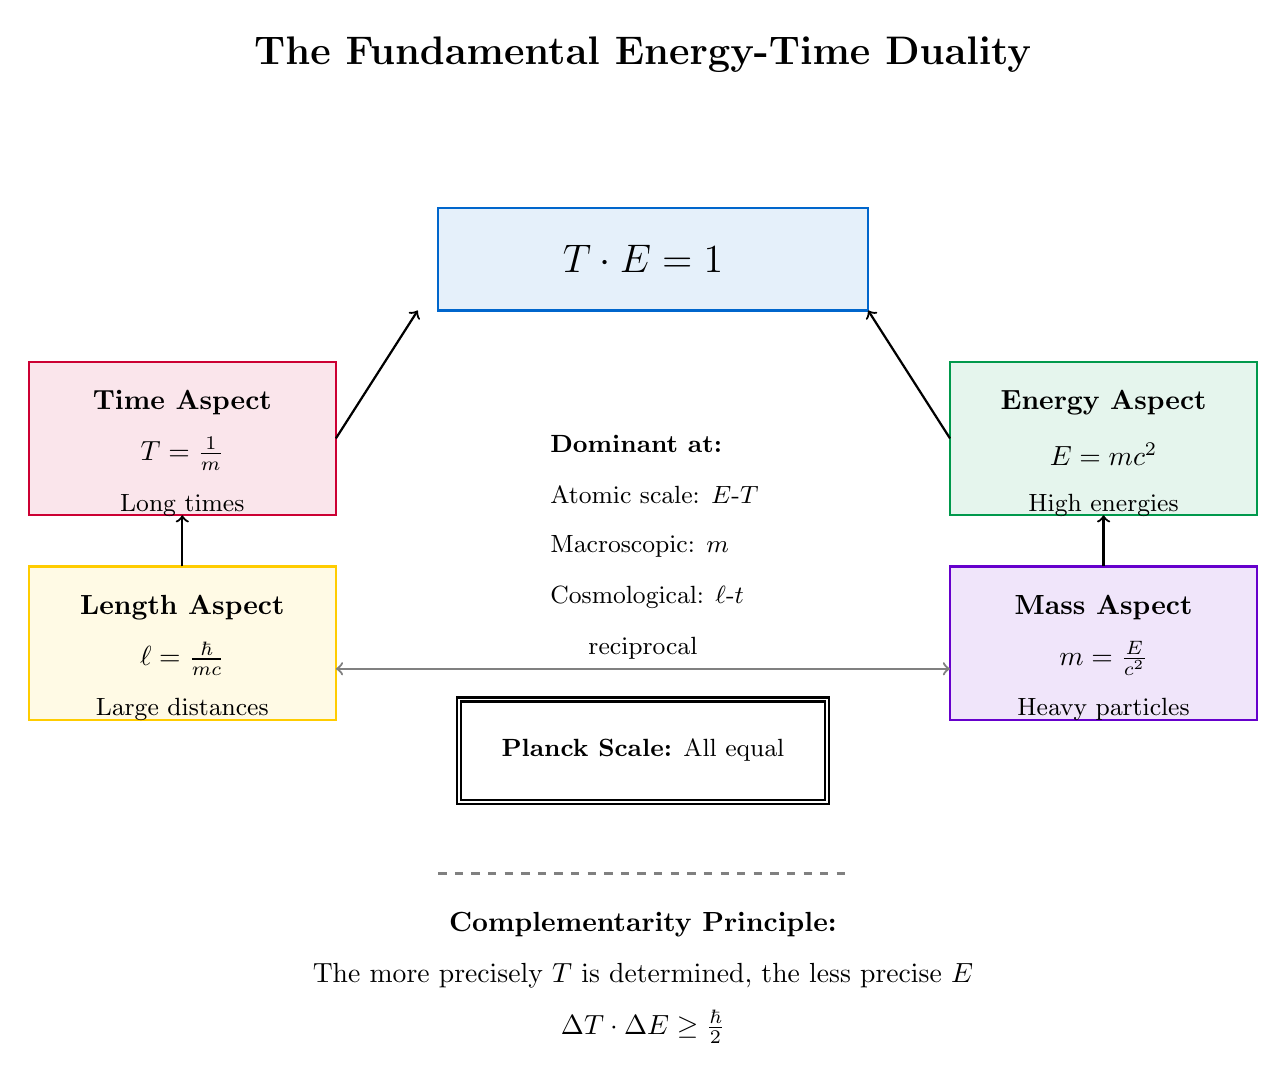
\begin{tikzpicture}[scale=1.3]
			% Title
			\node at (0, 6) {\Large \textbf{The Fundamental Energy-Time Duality}};
			
			% Main equation in center
			\draw[thick, t0blue, fill=t0blue!10] (-2, 3.5) rectangle (2.2, 4.5);
			\node at (0, 4) {\Large $T \cdot E = 1$};
			
			% Time side (left)
			\draw[thick, t0red, fill=t0red!10] (-6, 1.5) rectangle (-3, 3);
			\node at (-4.5, 2.6) {\textbf{Time Aspect}};
			\node at (-4.5, 2.1) {$T = \frac{1}{m}$};
			\node at (-4.5, 1.6) {\small Long times};
			\draw[thick, ->] (-3, 2.25) -- (-2.2, 3.5);
			
			% Energy side (right)
			\draw[thick, t0green, fill=t0green!10] (3, 1.5) rectangle (6, 3);
			\node at (4.5, 2.6) {\textbf{Energy Aspect}};
			\node at (4.5, 2.1) {$E = mc^2$};
			\node at (4.5, 1.6) {\small High energies};
			\draw[thick, ->] (3, 2.25) -- (2.2, 3.5);
			
			% Length relation (bottom left)
			\draw[thick, t0yellow, fill=t0yellow!10] (-6, -0.5) rectangle (-3, 1);
			\node at (-4.5, 0.6) {\textbf{Length Aspect}};
			\node at (-4.5, 0.1) {$\ell = \frac{\hbar}{mc}$};
			\node at (-4.5, -0.4) {\small Large distances};
			\draw[thick, ->] (-4.5, 1) -- (-4.5, 1.5);
			
			% Mass relation (bottom right)
			\draw[thick, t0purple, fill=t0purple!10] (3, -0.5) rectangle (6, 1);
			\node at (4.5, 0.6) {\textbf{Mass Aspect}};
			\node at (4.5, 0.1) {$m = \frac{E}{c^2}$};
			\node at (4.5, -0.4) {\small Heavy particles};
			\draw[thick, ->] (4.5, 1) -- (4.5, 1.5);
			
			% Complementarity (bottom)
			\draw[thick, dashed, gray] (-2, -2) -- (2, -2);
			\node at (0, -2.5) {\textbf{Complementarity Principle:}};
			\node at (0, -3) {The more precisely $T$ is determined, the less precise $E$};
			\node at (0, -3.5) {$\Delta T \cdot \Delta E \geq \frac{\hbar}{2}$};
			
			% Arrows for relationships
			\draw[thick, <->, gray] (-3, 0) -- (3, 0);
			\node[above] at (0, 0) {\small reciprocal};
			
			% Planck scale box
			\draw[thick, double, fill=white] (-1.8, -1.3) rectangle (1.8, -0.3);
			\node at (0, -0.8) {\small \textbf{Planck Scale:} All equal};
			
			% Scale dependence
			\node[right] at (-1, 2.2) {\small \textbf{Dominant at:}};
			\node[right] at (-1, 1.7) {\small Atomic scale: $E$-$T$};
			\node[right] at (-1, 1.2) {\small Macroscopic: $m$};
			\node[right] at (-1, 0.7) {\small Cosmological: $\ell$-$t$};
		\end{tikzpicture}
	\end{center}
	
	This diagram shows the fundamental energy-time duality and its connections to mass and length. The central relationship $T \cdot E = 1$ connects all aspects. Depending on the scale considered, different aspects of this duality dominate, but all are linked by the fundamental relationships.
	
	\subsection{The Fundamental Equivalences}
	
	In the T0 formalism, the basic physical quantities are linked by the following relationships:
	
	\begin{align}
		T \cdot E &= 1 \quad \text{(Time-Energy duality)} \\
		T &= \frac{1}{m} \quad \text{(Time-Mass relation)} \\
		E &= mc^2 \quad \text{(Mass-Energy equivalence)} \\
		\ell &= \frac{\hbar}{mc} = \frac{\hbar}{E/c} \quad \text{(Length as energy)}
	\end{align}
	
	These relationships show that lengths can also be interpreted as energy scales. The Compton wavelength $\lambda_C = \hbar/(mc)$ is the paradigmatic example: it represents the characteristic length scale at which the quantum nature of a particle with mass $m$ (or equivalently, energy $E = mc^2$) becomes manifest.
	
	\subsection{The Planck Scale as Universal Reference}
	
	All these dualities converge at the Planck scale:
	
	\begin{align}
		\lP &= \sqrt{\frac{\hbar G}{c^3}} \quad \text{(Planck length)} \\
		\tP &= \sqrt{\frac{\hbar G}{c^5}} \quad \text{(Planck time)} \\
		\mP &= \sqrt{\frac{\hbar c}{G}} \quad \text{(Planck mass)} \\
		\EP &= \sqrt{\frac{\hbar c^5}{G}} \quad \text{(Planck energy)}
	\end{align}
	
	Remarkably, these quantities satisfy the fundamental relationships:
	\begin{align}
		\tP \cdot \EP &= \hbar \\
		\lP &= c \cdot \tP \\
		\EP &= \mP c^2 \\
		\lP &= \frac{\hbar}{\mP c}
	\end{align}
	
	This consistency shows that the T0 dualities are not arbitrary but deeply rooted in the structure of spacetime.
	
	\section{Scale Dependence and Limits of Interpretation}
	
	T0 theory shows that the different aspects of duality—time, mass, energy, length—are differently pronounced depending on the scale considered. This scale dependence is fundamental and calls for caution when interpreting extreme situations.
	
	\subsection{Complementarity of Aspects}
	
	Different aspects dominate at different scales:
	\begin{itemize}
		\item \textbf{Planck scale:} All aspects are equivalent, no approximation valid
		\item \textbf{Atomic scale:} Energy-time duality dominates, gravity negligible
		\item \textbf{Macroscopic scale:} Mass aspect dominant, quantum effects suppressed
		\item \textbf{Cosmological scale:} Space-time structure dominant, local quantum effects irrelevant
	\end{itemize}
	
	\subsection{The Role of Small Corrections}
	
	Although the $\xi$ parameter ($\xi = 4/3 \times 10^{-4}$) and gravitational effects are often extremely small, they still have measurable effects. These small corrections are not negligible but essential for complete understanding:
	
	\begin{equation}
		\text{Observable effect} = \text{Main contribution} + \xi \cdot \text{Correction} + \text{Gravitational contribution}
	\end{equation}
	
	\subsection{Caution with Singularities}
	
	\begin{tcolorbox}[colback=t0yellow!10!white, colframe=t0yellow!75!black, title=Important Insight]
		Singularities are \textbf{not} the goal of T0 theory. They rather represent limits of applicability:
		\begin{itemize}
			\item As $r \to 0$: The local approximation breaks down
			\item As $E \to \infty$: The field equations become nonlinear
			\item As $T \to 0$: Time-energy duality loses its meaning
		\end{itemize}
		These limits show where the theory needs to be extended.
	\end{tcolorbox}
	
	\subsection{The Complementarity Principle in T0}
	
	Analogous to Bohr's complementarity principle in quantum mechanics, T0 theory states:
	
	\begin{equation}
		\text{Precision}(T) \times \text{Precision}(E) \leq \text{constant}
	\end{equation}
	
	The more precisely we determine one aspect (e.g., time), the less precise the complementary aspect (energy) becomes. This is not a weakness of the theory but a fundamental property of reality.
	
	\subsection{Interpretation Guidelines}
	
	For correct application of T0 theory, the following guidelines apply:
	
	\begin{enumerate}
		\item \textbf{Scale awareness:} Always check which scale is dominant
		\item \textbf{Take small effects seriously:} Don't ignore $\xi$ corrections and gravitational effects
		\item \textbf{Avoid singularities:} Understand them as hints at theoretical limits
		\item \textbf{Respect complementarity:} Not all aspects can be sharp simultaneously
		\item \textbf{Experimental verifiability:} Only make predictions that are measurable in principle
	\end{enumerate}
	
	\section{Resolution of Quantum Paradoxes}
	
	T0 theory offers elegant solutions to the classic paradoxes of quantum mechanics by showing that they result from an incomplete description of the underlying field structure.
	
	\subsection{Bell Correlations}
	
	The apparently instantaneous Bell correlations are resolved by T0 theory:
	
	\begin{itemize}
		\item \textbf{Local condition:} $T \cdot E = 1$ at both measurement locations
		\item \textbf{Shared field:} Entangled particles share field configuration
		\item \textbf{Causal propagation:} Field changes propagate with $c$
		\item \textbf{Correlation without communication:} Pre-structured field, no signal transmission
	\end{itemize}
	
	The crucial insight is that entangled particles are not correlated through mysterious instantaneous connections, but through a shared field established when they were created. This field exists throughout the spatial region and evolves causally according to the field equations. The observed correlations result from this pre-existing field structure, not instantaneous communication.
	
	\subsection{Wave Function Collapse}
	
	The supposedly instantaneous collapse is an illusion:
	\begin{align}
		\text{Measurement} &\rightarrow \text{Local field disturbance} \quad (t \sim t_{\text{Planck}}) \\
		&\rightarrow \text{Field propagation} \quad (v = c) \\
		&\rightarrow \text{Appears instantaneous since } t_{\text{Planck}} \ll t_{\text{meas}}
	\end{align}
	
	What appears as discontinuous collapse is actually a continuous process occurring on a time scale far below our measurement resolution. The measurement process is a local interaction between measuring device and field that creates a disturbance propagating causally.
	
	\section{Experimental Consequences}
	
	Although most T0 effects occur on immeasurably small time scales, the theory still makes testable predictions for extreme conditions.
	
	\subsection{Prediction of Measurable Delays}
	
	For cosmic Bell tests with distance $r$:
	\begin{equation}
		\Delta t_{\text{measurable}} = \xi \cdot \frac{r}{c}
	\end{equation}
	where $\xi = \frac{4}{3} \times 10^{-4}$ is the geometric parameter.
	
	\textbf{Numerical example:}
	\begin{itemize}
		\item Satellite experiment with $r = 1000$ km:
		\begin{equation}
			\Delta t = 1.333 \times 10^{-4} \times \frac{10^6 \text{ m}}{3 \times 10^8 \text{ m/s}} \approx 0.44 \, \mu\text{s}
		\end{equation}
		\item This delay is measurable with modern atomic clocks ($\Delta t_{\text{resolution}} \sim 10^{-9}$ s)
	\end{itemize}
	
	\subsection{Proposed Experiments}
	
	\begin{enumerate}
		\item \textbf{Satellite Bell test:} Entangled photons between ground station and satellite
		\item \textbf{Lunar laser ranging:} Precision measurement of quantum correlations Earth-Moon
		\item \textbf{Deep space quantum network:} Test at interplanetary distances
	\end{enumerate}
	
	\section{Philosophical Implications}
	
	The resolution of apparent instantaneity has profound consequences for our understanding of physical reality.
	
	\subsection{New Interpretation of Quantum Mechanics}
	
	T0 theory offers an alternative perspective on quantum mechanics:
	
	\begin{tcolorbox}[colback=t0red!5!white, colframe=t0red!75!black, title=New Perspective]
		\textbf{Standard interpretation:}
		\begin{itemize}
			\item Quantum mechanics requires non-locality
			\item Spooky action at a distance (Einstein)
			\item Wave function collapse
		\end{itemize}
		
		\textbf{T0 interpretation:}
		\begin{itemize}
			\item Everything is local in a shared field
			\item Correlations through field pre-structure
			\item Continuous, causal evolution
		\end{itemize}
	\end{tcolorbox}
	
	This paradigm shift solves many conceptual problems that have plagued quantum mechanics since its inception. The need for different interpretations disappears when one recognizes that the apparent paradoxes result from an incomplete description.
	
	\subsection{Unification of Quantum Mechanics and Relativity}
	
	T0 theory resolves the apparent conflict:
	\begin{itemize}
		\item Preserves Lorentz invariance completely
		\item No faster-than-light information transmission
		\item Quantum correlations through causal field structure
	\end{itemize}
	
	This unification is not just formal but conceptual. Both theories are understood as different aspects of the same underlying field structure. Quantum mechanics describes the coherent properties of fields, while relativity characterizes their causal structure.
	
	\section{The Measurement Process in Detail}
	
	The measurement process in quantum mechanics has always been one of the greatest conceptual problems. Wave function collapse appears to be a non-unitary, instantaneous process fundamentally different from normal Schrödinger evolution. The T0 formalism offers an alternative description that avoids these problems.
	
	In the T0 picture, a measurement is a local interaction between the measuring device and the field at the measurement location. This interaction occurs on the Planck time scale—extremely fast but not instantaneous. The apparent collapse is actually a very rapid but continuous reorganization of the local field structure.
	
	Crucially, this local reorganization does not require instantaneous change of the field at distant locations. Information about the measurement propagates as a field disturbance at the speed of light. When this disturbance reaches other parts of an entangled system, it influences their further evolution, but this happens causally and at finite speed.
	
	This description eliminates the conceptual problems of the measurement process. There is no mysterious collapse, no violation of unitarity, and no instantaneous action at a distance. Everything is described by local field interactions and causal field propagation.
	
	\section{Quantum Entanglement Without Instantaneity}
	
	Quantum entanglement is often considered the paradigmatic example of non-local quantum phenomena. When two particles are entangled, measurement of one particle seems to instantly determine the state of the other, regardless of distance. Bell's inequalities and their experimental violation seem to prove that local realistic theories cannot reproduce quantum mechanics.
	
	The T0 formalism offers a new perspective on these phenomena. Entanglement is not interpreted as a mysterious instantaneous connection but as the result of a shared field configuration established when the entangled particles were created. This field configuration exists throughout the spatial region between the particles and evolves according to causal field equations.
	
	When a measurement is performed on one of the entangled particles, the measuring apparatus interacts locally with the field at that location. This interaction creates a disturbance in the field that propagates at the speed of light. The correlations between measurement results arise not from instantaneous communication but from the pre-existing structure of the shared field.
	
	This interpretation resolves the EPR paradox in a way fully compatible with both quantum mechanics and relativity. There is no spooky action at a distance, only local interactions with an extended field. The observed correlations result from coherent field structure, not instantaneous information transmission.
	
	\section{Summary and Outlook}
	
	The analysis of the T0 formalism clearly shows that the apparent instantaneity of quantum mechanics is an illusion arising from several factors.
	
	\subsection{Central Results}
	
	T0 theory eliminates instantaneity through a hierarchical structure:
	
	\begin{enumerate}
		\item \textbf{Local level:} $T \cdot E = 1$ as constraint condition (no dynamics)
		\item \textbf{Field level:} Wave equation with propagation $v \leq c$ (causal dynamics)
		\item \textbf{Measurable level:} Appears instantaneous because $\Delta t < $ resolution
	\end{enumerate}
	
	This hierarchy is key to understanding why quantum mechanics appears non-local while the underlying physics remains completely local and causal.
	
	\subsection{The Fundamental Insight}
	
	\begin{tcolorbox}[colback=t0yellow!10!white, colframe=t0yellow!75!black, title=Core Message]
		The apparent instantaneity of quantum mechanics is an illusion arising from:
		\begin{itemize}
			\item The notation of local constraint conditions
			\item The extreme smallness of Planck time
			\item The pre-structuring of shared fields
		\end{itemize}
		T0 theory shows that all phenomena are strictly causal and local when the complete field dynamics is considered.
	\end{tcolorbox}
	
	The implications of this insight extend far beyond technical details. It shows that nature, despite its quantum character, is fundamentally understandable and causally structured. The apparent mysteries of quantum mechanics dissolve when one takes the right theoretical perspective.
	
	\subsection{Outlook}
	
	T0 theory opens new research directions:
	\begin{itemize}
		\item Precision tests of predicted delays
		\item Quantum information theory with field correlations
		\item Cosmological implications of time field dynamics
		\item Technological applications in quantum communication
	\end{itemize}
	
	Each of these directions promises new insights into the fundamental nature of reality. T0 theory is not just a mathematical reformulation but a new conceptual foundation for our understanding of the quantum world. The resolution of apparent instantaneity is an important step in the further development of our physical worldview.
	
	The future of physics may lie in recognizing that the apparent mysteries of the quantum world are not fundamental but result from an incomplete description. T0 theory shows a path to a more complete understanding in which locality, causality, and observed quantum phenomena coexist harmoniously.
	
	\begin{thebibliography}{99}
		\bibitem{t0_foundations}
		T0 Theory Foundations (2024). \textit{Time-Mass Duality and Geometric Field Theory}. Internal Research Document.
		
		\bibitem{bell_original}
		Bell, J.S. (1964). On the Einstein Podolsky Rosen Paradox. \textit{Physics Physique Fizika}, \textbf{1}, 195--200.
		
		\bibitem{einstein_epr}
		Einstein, A., Podolsky, B., Rosen, N. (1935). Can Quantum-Mechanical Description of Physical Reality Be Considered Complete? \textit{Physical Review}, \textbf{47}, 777--780.
		
		\bibitem{aspect_experiments}
		Aspect, A., Grangier, P., Roger, G. (1982). Experimental Realization of Einstein-Podolsky-Rosen-Bohm Gedankenexperiment. \textit{Physical Review Letters}, \textbf{49}, 91--94.
		
		\bibitem{planck_units}
		Planck, M. (1899). Über irreversible Strahlungsvorgänge. \textit{Sitzungsberichte der Preußischen Akademie der Wissenschaften}, 440--480.
	\end{thebibliography}
	
\end{document}